\documentclass[11pt,a4paper,english]{article}
  \usepackage[latin1]{inputenc}
  \usepackage{amsmath,amsfonts,amssymb}
  \usepackage{enumitem}
  \usepackage{fullpage}
  \usepackage{graphicx}
  \usepackage{tabto}
  \usepackage{etoolbox}
  \usepackage{hyperref}
  \usepackage{minted}
  \usepackage{parskip}
  \usepackage[ruled,linesnumbered,noline,noend]{algorithm2e}
  \usepackage[font=small,labelfont=bf]{caption}
  \newcommand\numberthis{\addtocounter{equation}{1}\tag{\theequation}}
  \renewcommand{\labelenumii}{\theenumii}
  \renewcommand{\theenumii}{\theenumi.\arabic{enumii}.}

  \title{Algorithmic Methods of Data Mining - Assignment 3}
  \author{Maksad Donayorov}

  \begin{document}
    \maketitle
    \definecolor{bg}{rgb}{0.95,0.95,0.95}

    \section{Problem. \textit{Clustering given a hierarchy:}}
      \subsection{
        \textit{k-means on trees can be solved optimally in polynomial time}
      }
        To prove the k-means on tree can be solved optimally in polynomial time let's start by stating a pseudocode that solves this problem and then discuss how it works:
        \begin{minted}[bgcolor=bg,linenos,fontsize=\small,autogobble]{python}
          optimal_clusters = []
          for node in TraversalPostorder(tree):
            if node does not have children:
              tuple = (1, 0, [node.index], [node.value])
              optimal_clusters.append(tuple)
            if node has children:
              children = node.left_child + node.right_child
              numb_of_clusters = children.clusters
              node_self = (
                numb_of_clusters,
                calc_self_var,
                [children.indices],
                [children.elements]
              )
              tuple = (node_self, children)
              optimal_clusters.append(tuple)
            tuple.filter_the_optimal
          tuple.trim_elements
        \end{minted}

        Assume that we have a tree like this:
        \begin{minted}[bgcolor=bg,fontsize=\small,autogobble]{text}
               1
             /   \
            2     3
          /   \
         4     5
        \end{minted}
        Then the $TraversalPostorder(tree)$ will run as:
        \begin{minted}[bgcolor=bg,fontsize=\small,autogobble]{text}
          4 5 2 3 1
        \end{minted}

        This allows us to travel through the tree only once. Based on the pseudocode we should not need to refer to the children, once we have computed the needed parameters. The main idea in here is that we create a $tuple$ of the needed parameters when we are visiting a node or a leaf, store all of the parameters and move to the next. For instance, at line 4:
        \begin{minted}[bgcolor=bg,fontsize=\small,autogobble]{python}
          tuple = (1, 0, [node.index], [node.value])
        \end{minted}
        We ar creating the tuple out of a leaf. The first parameter of that $tuple$ is an indicator of clusters and since a leaf can only have a cluster of one element, it's default value is 1. \\
        The second parameter of that tuple is $0$, that indicates the variance at that point. Again, since there is no more than one element at the leaf the variance will be $0$. \\
        The third element is an array of indices, we need that for later. \\
        The fourth parameter is the an array of element that that leaf holds. This will be needed once we are in the parent node and want to compute the variance.\\
        After we do the computation at the first leaf we move to the next leaf and eventually to the parent where we compute the parameters (later in the example these parameters are noted as tuples).
        This sounds very complicated and indeed it is, as there isn't a better approach I came up with. Let's look into more concrete example hope to make things more clear. Let's assume that we have this tree with given leaves:
        \begin{minted}[bgcolor=bg,fontsize=\small,autogobble]{text}
                v1
              /   \
            v2     v3
           /  \   /  \
          2    4 v4   \
                /  \   \
               3   7   12
        \end{minted}

        In this tree we have $n=5$ and the leaves are 2, 4, 3, 7, 12. We have 4 "layers" and we can compute the variance, number of clusters and number of vertices. The first thing we do is to compute the level $I$ as that's the easiest (please note that we are not following at this point the postorder's steps to simplicity reason). This is how it looks like:
        \begin{center}
          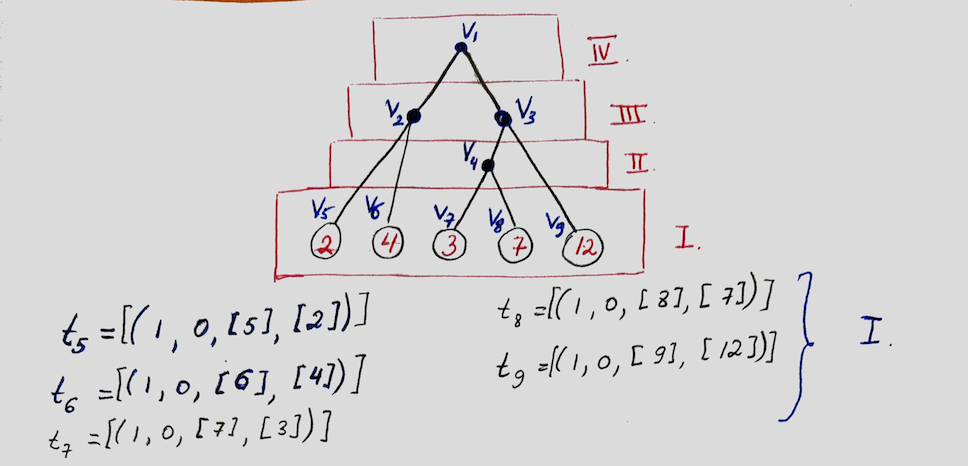
\includegraphics[width=15cm]{sc_1.png}
        \end{center}
        Here we create tuples for each leaf. For example, the:
        \begin{minted}[bgcolor=bg,fontsize=\small,autogobble]{python}
          t5 = (1, 0, [5], [2])
        \end{minted}

        means that this is the vertex 5, that has one "cluster", it's index is 5 and the elements that it holds are [2]. With that representation we can move to the second and third "levels". \\
        It is a bit tricky to calculate the tuples for nodes. That's because the nodes have 2 combinations:
        \begin{enumerate}
          \item When we are clustering the elements in the node (let's denote it by $t_{self}$).
          \item When we are clustering the elements in the children nodes/leaves ($t_{left} + t_{rigth}$).
        \end{enumerate}

        Let's now calculate the parameters ($t_2$) for $vertex_2$:
        \begin{center}
          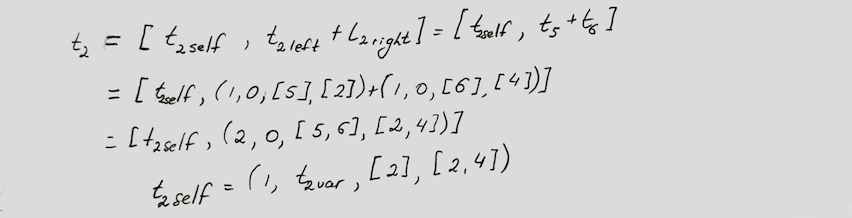
\includegraphics[width=15cm]{sc_2.png}
        \end{center}

        Now that we have calculated the left and the rigth children of $t_2$, we need to find the variance at $t_2$ that will be used for $t_{self}$:
        \begin{center}
          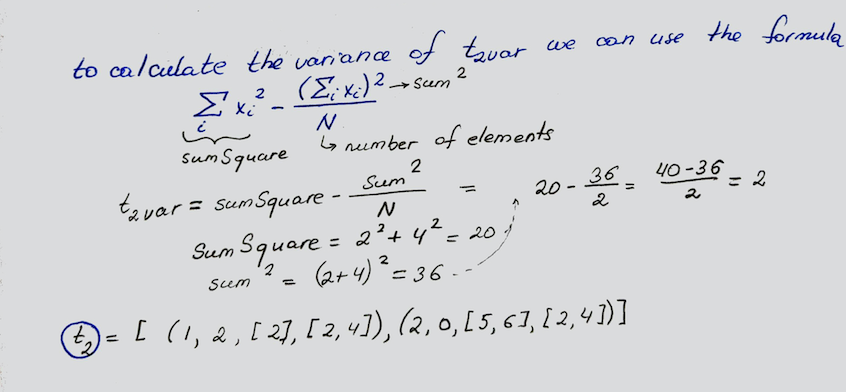
\includegraphics[width=15cm]{sc_3.png}
        \end{center}

        As you might have noticed we are not using the formula that is given in the problem description to calculate the variance. Instead, we are using a more efficient formula that relies on number of elements, sum of the elements and "square sum" of those elements (\href{https://math.stackexchange.com/questions/20593/calculate-variance-from-a-stream-of-sample-values}{link to the formula}).

        Now we can move to the next vertex and certainly the same logic applies:
        \begin{center}
          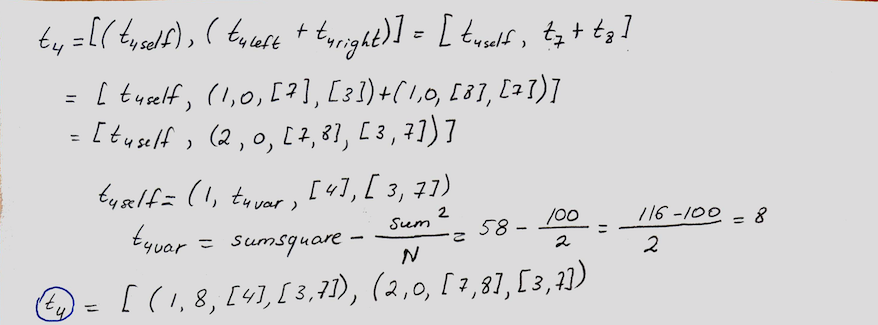
\includegraphics[width=15cm]{sc_4.png}
        \end{center}

        Please pay attention to the summation of left and right children that have more than one tuple:
        \begin{center}
          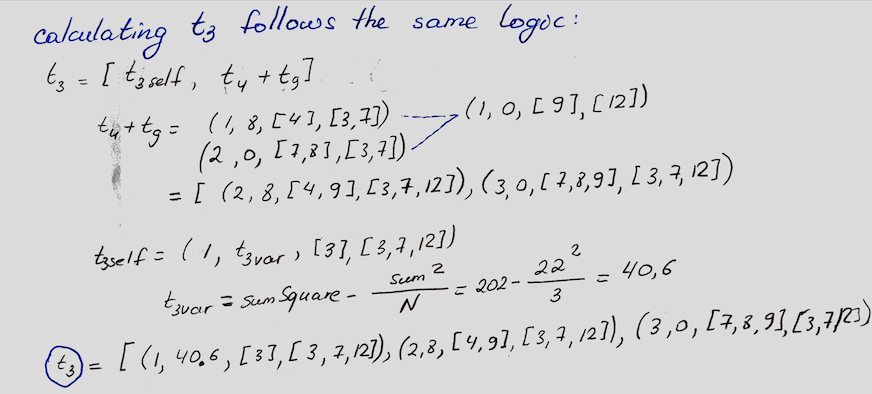
\includegraphics[width=15cm]{sc_5.png}
        \end{center}

        Up to this point we have computed all the parameters (tuples) for the all the children. Now, it's time to calculate them for $vertex_1$.
        \begin{center}
          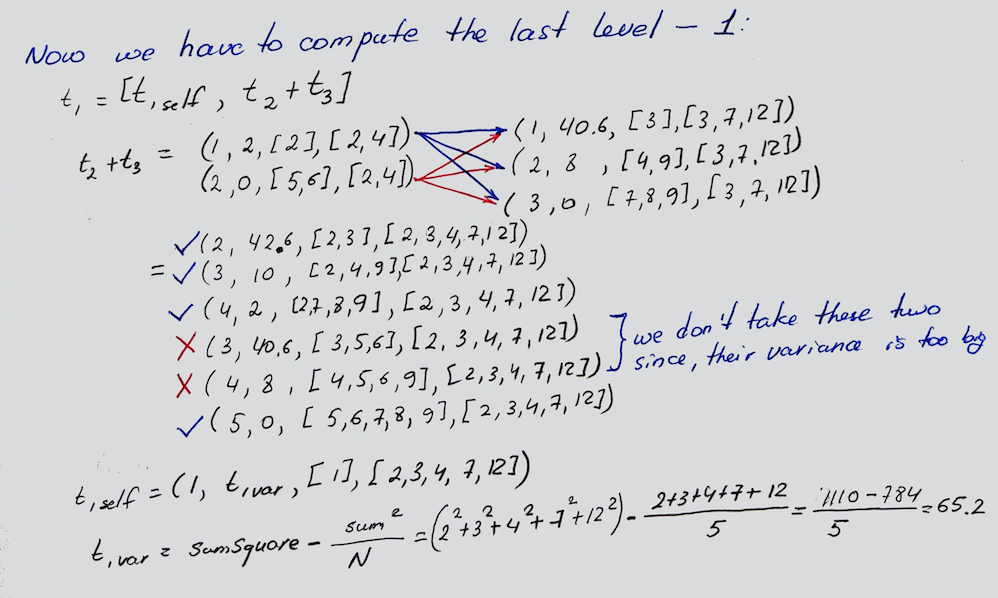
\includegraphics[width=15cm]{sc_6.png}
        \end{center}
        A very important point in the above calculation is how we choose some of the tuples. As you can see, those tuples that we choose are marked with the blue tick and those which are not chosen marked by red cross. This implies that we have 2 clusters with the same value of $k$ and we only choose the optimal one, which is a tuple with the smaller variance. In the pseudocode that's done on line 16.

        The final version of the $t_1$ looks like this:
        \begin{center}
          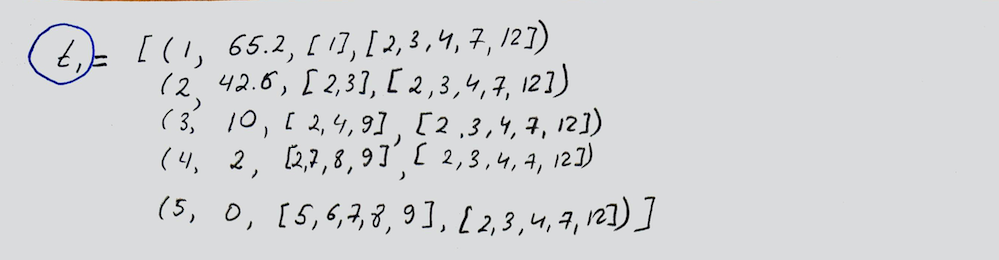
\includegraphics[width=15cm]{sc_7.png}
        \end{center}

        The final result that our algorithm returns is a list of the tuples with all the possible combination of clusters where $1 \leq k \leq 5$. Looking at this table we can immediately tell what is the optimal cluster, what kind of vertices it will have and what is its variance (the elements are that each tuple holds are trimmed at line 17 of the pseudocode):
        \begin{minted}[bgcolor=bg,fontsize=\small,autogobble]{text}
          [
            (1, 65.2, [1],           ),
            (2, 42.6, [2, 3],        ),
            (3, 10,   [2, 4, 9],     ),
            (4, 2,    [2, 7, 8, 9],  ),
            (5, 0,    [5, 6, 7, 8, 9])
          ]
        \end{minted}

        For example, if $k=3$, we can say that the optimal cluster will have variance of $10$ with vertices indices of [2, 4, 9]:
        \begin{minted}[bgcolor=bg,fontsize=\small,autogobble]{text}
               v1
              /   \
            v2     v3
                  /  \
                 v4   12
        \end{minted}

        Or if $k=4$, then the optimal cluster will have a variance of 2 with vertices [2, 7, 8, 9]:
        \begin{minted}[bgcolor=bg,fontsize=\small,autogobble]{text}
                v1
              /   \
            v2    v3
                 /  \
                v4   \
               /  \   \
              3    7  12
        \end{minted}

      \subsection{
        \textit{correctness of this algorithm}
      }
        As we have seen the algorithm returns only the optimal "tuples" with the optimal number of clusters. Therefore, it will always filter the tuples that have a bigger variance (see line 17 of the pseudocode) before moving to the next step. For example, suppose that we have $k=3$ and the list of tuples looks like this:
        \begin{minted}[bgcolor=bg,fontsize=\small,autogobble]{text}
          (3, 10,   [2, 4, 9],  [2, 3, 4, 7, 12])
          (3, 40.6, [3, 5, 6],  [2, 3, 4, 7, 12])
        \end{minted}
        Then the algorithm will return the $t$ with the smallest variance, which is in this case $10$:
        \begin{minted}[bgcolor=bg,fontsize=\small,autogobble]{text}
          (3, 10,   [2, 4, 9],  [2, 3, 4, 7, 12])
        \end{minted}

        For detailed explanation of the correctness of this algorithm, please look at the at \textbf{section 1.1}.

      \subsection{
        \textit{complexity of the algorithm}
      }
        There are 3 main component to this algorithm that we have to take into consideration when calculate the complexity of it.
        \begin{enumerate}
          \item The \textit{Postorder Traversal} algorithm that we are using, which has complexity of $\mathcal{O}(n)$.
          \item Number of computation of tuples $t$.
          \item The variance for each $t$.
        \end{enumerate}

        Let's start with the variance. We are using a formula that has a complexity of $4n$:
        \begin{align*}
          \sum_i x_i^2 - \frac{(\sum_i x_i)^2}{N}
        \end{align*}
        We are using that formula for each tuple. The number of times $t$ is calculated equals to $2n-1$. $n$ times for the leaves and $n-1$ times for the parent nodes. \\
        So in total, $t$ and $variance$ with the \textit{Postorder Traversal algorithm} are calculated $n(4n^2-4n) = 4n^3-4n^2$ times.\\
        Consequently, the complexity of this algorithm is $\mathbf{\mathcal{O}(n^3)}$.

    \section{Clustering a data stream}
      \subsection{Prove of SF algorithm produces a clustering that has at most $k$ cluster centers.}
        We can prove that the Streaming-Furthest algorithm produces a clustering that has at most $k$ cluster centers, by contradiction. Let's assume that the algorithm produces more clusters than the optimal, which can pe denoted by $p > k$. Where $k$ is the number of clusters that was produced by the optimal and $p$ is the number cluster that were produced by the algorithm. In other words:
        \begin{align*}
          C^* & = \{C_1, C_2, C_3 ... C_k\} - optimal\ case \\
          Ac & = \{Ac_1, Ac_2, Ac_3 ... Ac_p\} - algorithm\ case \\
          & where \ p > k
        \end{align*}
        In this case there will be at least two centers: $\{s_1, s_2\} \in Ac $, that lie inside one of the cluster found in the optimal $C^*$.
        The representation and depiction of this statement will look like this:
        \begin{center}
          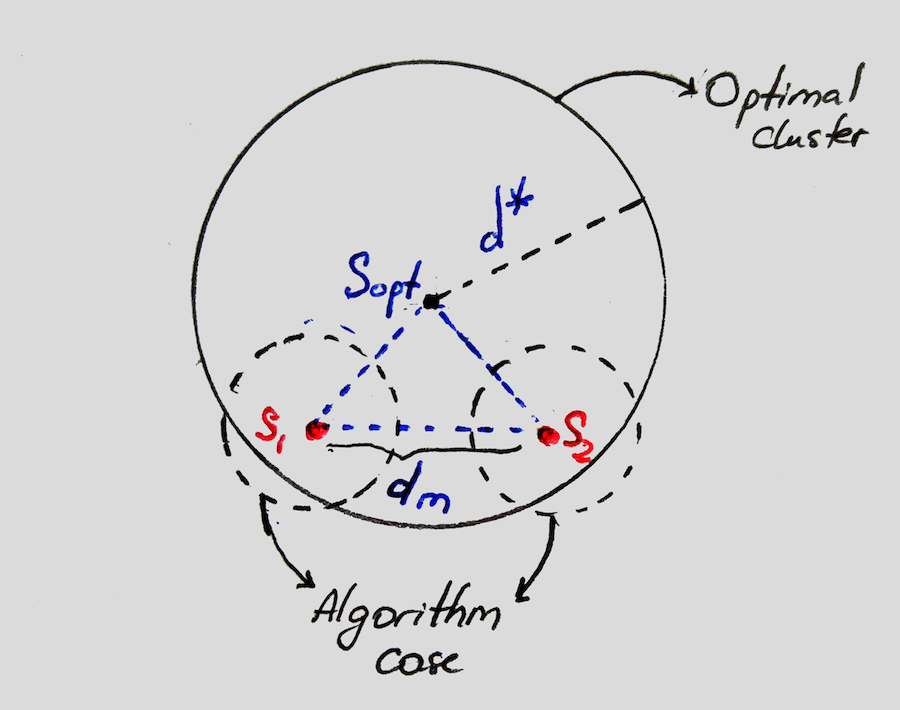
\includegraphics[width=7cm]{sc_8.png}
        \end{center}
        From here we can make our analogy that:
        \begin{align*}
          d(s_1, s_2) \leq d(s_1, S_{opt}) + d(s_2, S_{opt}) \leq 2d^*
        \end{align*}
        From the above inequality we can see that $d(s_1, s_2) \leq 2d^*$ and based on the algorithm this cannot happen. Because, in the algorithm the cluster centers are assigned with the condition that $d_m > 2d^*$. Consequently, we prove by contradiction that the Streaming-Furthest algorithm produces a clustering that has at most $k$ clusters.
      \subsection{Prove of SF algorithm is still a factor-2 approximation.}
        At the very beginning when the first element arrives it becomes a center of a new cluster. When the next element comes then we check if it is $2d^*$ apart or not. Since all the points that are coming from the data stream will go through the condition $d_m > d2^*$, we can either assign them to be an element of an already existing cluster or a center of a new cluster. The center assignment is done only if the condition $d_F \leq 2d^*$ is satisfied. At the very end, when all elements are streamed we will end up in a situation that all the elements that are not center are at most $2d^*$ apart from their closest cluster. Consequently, the maximum radius of a cluster or the cost of clustering is less than or equal to $2d^*$. That being said, we can conclude that the SF algorithm is a factor-2 approximation.
      \subsection{Modification of the SF algorithm.}

        \begin{algorithm}
          \caption{modified version of the the STREAMING-FURTHEST algorithm without known $d^*$}
          \KwIn{
            a stream of data points X\\
            (the optimal k-centers cost $d^*$ is NOT known)
          }
          \KwOut{clustering of points in X in k clusters}
          \While{read from the stream $\{x_1, x_2 ... x_k\}$}{
            initialize clusters centers $C \gets \{x_1, x_2 ... x_k\}$; \\
            initialize the optimal radius to be the longest distance between clusters' centre divide by 2:  $d^* \gets max(distance(C))/2$
          }

          \While{read from the stream $x_i \gets \{x_{k+1}, x_{k+2}, x_{k+3}...\}$}{
            find the closest cluster center to the next element: $c_{closest} \gets closest(x_i, C)$; \\
            compute the distance to the closest cluster $d_m \gets distance(c_{closest})$; \\
            \uIf {$d_m > d^*$}{
              update the optimal distance: $d^* \gets d^* + d_m$; \\
              remove the closest cluster center and add new cluster center:
              $C \gets C.remove(c_{closest}) \ \& \ C.add(x_i)$ \\
              assign $c_{closest}$ to the new cluster center (which is $x_i$)
            }
            \Else {
              assign $x_i$ to its closest cluster center (which is $c_{closest}$)
            }
          }
          \KwRet{return the set C of cluster centers}
        \end{algorithm}

        This algorithm is certainly not the best out there, but it does compute $k$ clusters without known $d^*$. I won't prove the correctness of it, as it is not specified as a requirement in the problem description. One downside of the algorithm is that the radius eventually becomes quite large, which is fine in this case. This is due to the fact that elements are assigned to the cluster by the closest distance and if the radii of all of the clusters do not cover the next element, then it becomes a new cluster center and we recompute the optimal distance $d^*$.

    \section{Problem}
      \subsection{Propose a streaming algorithm.}

        \begin{minted}[bgcolor=bg,linenos,fontsize=\small,autogobble]{python}
          '''
          Input: stream of edges
          Output: bolean at a given time. True if graph is connected and
          False if graph is disconnected
          '''
          vertices = set([])
          edges = []
          while 'streaming is active':
            edge = 'read the next edge'
            if len(edges) == W:
              #remove the oldest edge from edges
              edges.pop(0)

            edges.append(edge)
            vertices.add(edge.vertices)

            bredth_first_search.init(edges):
            if bredth_first_search.cycle:
              edges = bredth_first_search.remove_cycles_oldest_edge

            if len(vertices) - len(edges) == 1:
              return True
            else:
              return False
        \end{minted}
        (\href{https://en.wikipedia.org/wiki/Breadth-first_search}{link to Breadth-first search algorithm}).

      \subsection{Correctness of the algorithm.}
        We know that if the difference of number of edges and number of vertices is 1, then we can say that the graph is connected. In order for us to apply this to our case, where edges coming as stream, we need to ensure that our graph has no cycle and we brake the loop as soon as it forms. The main idea behind this logic is that we remove the oldest edge that is in a cycle, as it will be removed eventually. For example, we have sliding window with length 5, edges \textit{\{(a,b)(b,c),(a,c),(a,d),(d, e)\}}  and our graph looks like this:
        \begin{minted}[bgcolor=bg,fontsize=\small,autogobble]{text}
               a
             /   \
            b --- c
                   \
              e --- d
        \end{minted}
        we can immediately see the formed loop between \textit{\{a, b, c\}} without waiting for the new edge to arrive. In this case we remove the "oldest" edge of the cycle and our graph will look like this:
        \begin{minted}[bgcolor=bg,fontsize=\small,autogobble]{text}
                a
                 \
            b --- c
                   \
              e --- d
        \end{minted}
        And once the new edge arrives, let's suppose it is \textit{(b, e)}, then we first add the edge, check for cycle and if it exist, then remove it:
        \begin{minted}[bgcolor=bg,fontsize=\small,autogobble]{text}
                a
                 \
            b --- c
             \     \
              e --- d
        \end{minted}
        Now that we added \textit{(b,e)} and we found a new cycle, \textit{(b,c,d,e)}, we can break that cycle. Our algorithm will check the oldest edge and remove it. In this case it is \textit{(b,c)}:
        \begin{minted}[bgcolor=bg,fontsize=\small,autogobble]{text}
                a
                 \
            b     c
             \     \
              e --- d
        \end{minted}
        With that we can ensure that the graph is still connected, but it has no loop. \\
        Let's assume that the next edge that comes is \textit{(e, f)}. In that case we add the new edge and do not remove anything as the number of edges in the sliding window is equal to 5 and there is no any cycle:
        \begin{minted}[bgcolor=bg,fontsize=\small,autogobble]{text}
                a
                 \
            b     c
             \     \
              e --- d
               \
                f
        \end{minted}
        Let's add one final case to test the "disconnectivity" of the graph. Suppose the next edge will be \textit{(f,g)}. We then add this new ege and remove the oldest edge, (which is \textit{(a,c)}). Our graph will be then disconnected, as it is supposed to be:
        \begin{minted}[bgcolor=bg,fontsize=\small,autogobble]{text}
                a

            b     c
             \     \
              e --- d
               \
                f --- g
        \end{minted}
        As you can see the algorithm does cover all the cases. It does show when the graph is connected or when it is not.

      \subsection{Space that the algorithm uses.}
        The space complexity of the algorithm is: $\mathcal{O}(n * k)$. \textit{n} here is an indication for sliding window and k for bredth first search.

      \subsection{Update time of the algorithm.}
        The time complexity of the algorithm is also $\mathcal{O}(n * k)$. \textit{n} here is an indication for sliding window and k for bredth first search.
\end{document}

